\chapter{ملاحظة العالم: الحواس الخمس}\label{ch:g1:five-senses}

يغرّد طائر في مكان ما فوقك. ورائحة الخبز دافئة. والبلاط بارد تحت
جوربيك. قبل أي شيء آخر، تنظر الفيزياء وتُصغي وتلمس: هذا الفصل عن
\omterm{def:g1:five-senses:observation}{ملاحظة} العالم بالحواس الخمس --- وعن الحيل التي تخدعنا بها أحيانًا.

\section{الحواس الخمس}

\begin{definition}[الحواس الخمس]\label{def:g1:five-senses:senses}
\emph{الحاسّة}\index{حاسّة} طريقة يعرف بها الجسم ما يجري في
العالم. ولنا خمس حواس:
\begin{enumerate}
  \item \emph{البصر}\index{بصر} --- العينان تريان الضوء والألوان
        والأشكال؛
  \item \emph{السمع}\index{سمع} --- الأذنان تسمعان الأصوات؛
  \item \emph{اللمس}\index{لمس} --- الجلد يحسّ بالخشن والناعم،
        وبالدافئ والبارد؛
  \item \emph{الشمّ}\index{شمّ} --- الأنف تشمّ الخبز الدافئ؛
  \item \emph{الذوق}\index{ذوق} --- اللسان يذوق الحلو والمالح
        والحامض.
\end{enumerate}
\end{definition}

\begin{omfigure}
\begin{tikzpicture}[scale=0.8]
  \foreach \x/\name in {0/البصر, 2.4/السمع, 4.8/اللمس, 7.2/الشمّ,
      9.6/الذوق} {
    \draw[thick, omDef] (\x,0) circle (0.9);
    \node[below, font=\small] at (\x,-1.1) {\name};
  }
  % eye
  \draw[thick] (0,0) ellipse (0.55 and 0.3);
  \fill[omDef] (0,0) circle (0.18);
  \fill (0,0) circle (0.09);
  \fill[white] (0.06,0.07) circle (0.03);
  % ear: outer contour over the top, down to the lobe, plus inner ridge
  \draw[thick] (2.12,0.3)
    .. controls (2.1,0.62) and (2.42,0.72) .. (2.66,0.52)
    .. controls (2.88,0.32) and (2.86,-0.08) .. (2.68,-0.32)
    .. controls (2.55,-0.5) and (2.4,-0.62) .. (2.26,-0.6)
    .. controls (2.1,-0.58) and (2.06,-0.42) .. (2.14,-0.32);
  \draw[thick] (2.24,0.28)
    .. controls (2.26,0.46) and (2.5,0.5) .. (2.6,0.32)
    .. controls (2.7,0.12) and (2.64,-0.08) .. (2.5,-0.16);
  % hand print: palm and five fingers
  \fill[omDef!30] (4.72,-0.22) ellipse (0.34 and 0.28);
  \draw[thick] (4.72,-0.22) ellipse (0.34 and 0.28);
  \foreach \a/\r in {135/0.5, 108/0.56, 84/0.58, 60/0.54} {
    \fill[omDef!30] (4.72,-0.22) ++(\a:\r)
      ellipse [x radius=0.085, y radius=0.17, rotate=\a-90];
    \draw[thick] (4.72,-0.22) ++(\a:\r)
      ellipse [x radius=0.085, y radius=0.17, rotate=\a-90];
  }
  \fill[omDef!30] (4.72,-0.22) ++(170:0.46)
    ellipse [x radius=0.08, y radius=0.14, rotate=60];
  \draw[thick] (4.72,-0.22) ++(170:0.46)
    ellipse [x radius=0.08, y radius=0.14, rotate=60];
  % nose in profile: brow, bridge sloping down-left, rounded tip,
  % nostril wing curling back
  \draw[thick] (7.5,0.62)
    .. controls (7.32,0.4) and (7.16,0.14) .. (7.1,-0.08)
    .. controls (7.05,-0.26) and (7.14,-0.4) .. (7.3,-0.4)
    .. controls (7.4,-0.4) and (7.46,-0.34) .. (7.46,-0.26);
  \draw[thick] (7.46,-0.26)
    .. controls (7.56,-0.3) and (7.6,-0.42) .. (7.5,-0.48)
    .. controls (7.42,-0.53) and (7.3,-0.49) .. (7.28,-0.42);
  \fill (7.38,-0.44) ellipse (0.05 and 0.033);
  % lips
  \draw[thick] (9.2,0.06) .. controls (9.4,0.24) and (9.52,0.12) ..
    (9.6,0.16) .. controls (9.68,0.12) and (9.8,0.24) .. (10.0,0.06);
  \draw[thick] (9.2,0.06) .. controls (9.45,-0.28) and (9.75,-0.28)
    .. (10.0,0.06);
  \draw[thick] (9.34,0.02) .. controls (9.6,-0.08) .. (9.86,0.02);
\end{tikzpicture}

{\small الحواس الخمس: العين والأذن واليد والأنف واللسان --- خمسة
أبواب بين العالم وبينك.}
\end{omfigure}

\begin{example}[تفاحة واحدة وخمس حواس]\label{ex:g1:five-senses:apple}
أكل تفاحة يستعمل الحواس كلها: \emph{ترى} قشرتها الحمراء،
و\emph{تحسّ} بها ملساء مستديرة في يدك، و\emph{تسمع} صوت القضمة،
و\emph{تشمّ} عطرها، و\emph{تذوق} عصيرها الحلو. خمس حواس وتفاحة
واحدة.
\end{example}

\begin{omfigure}
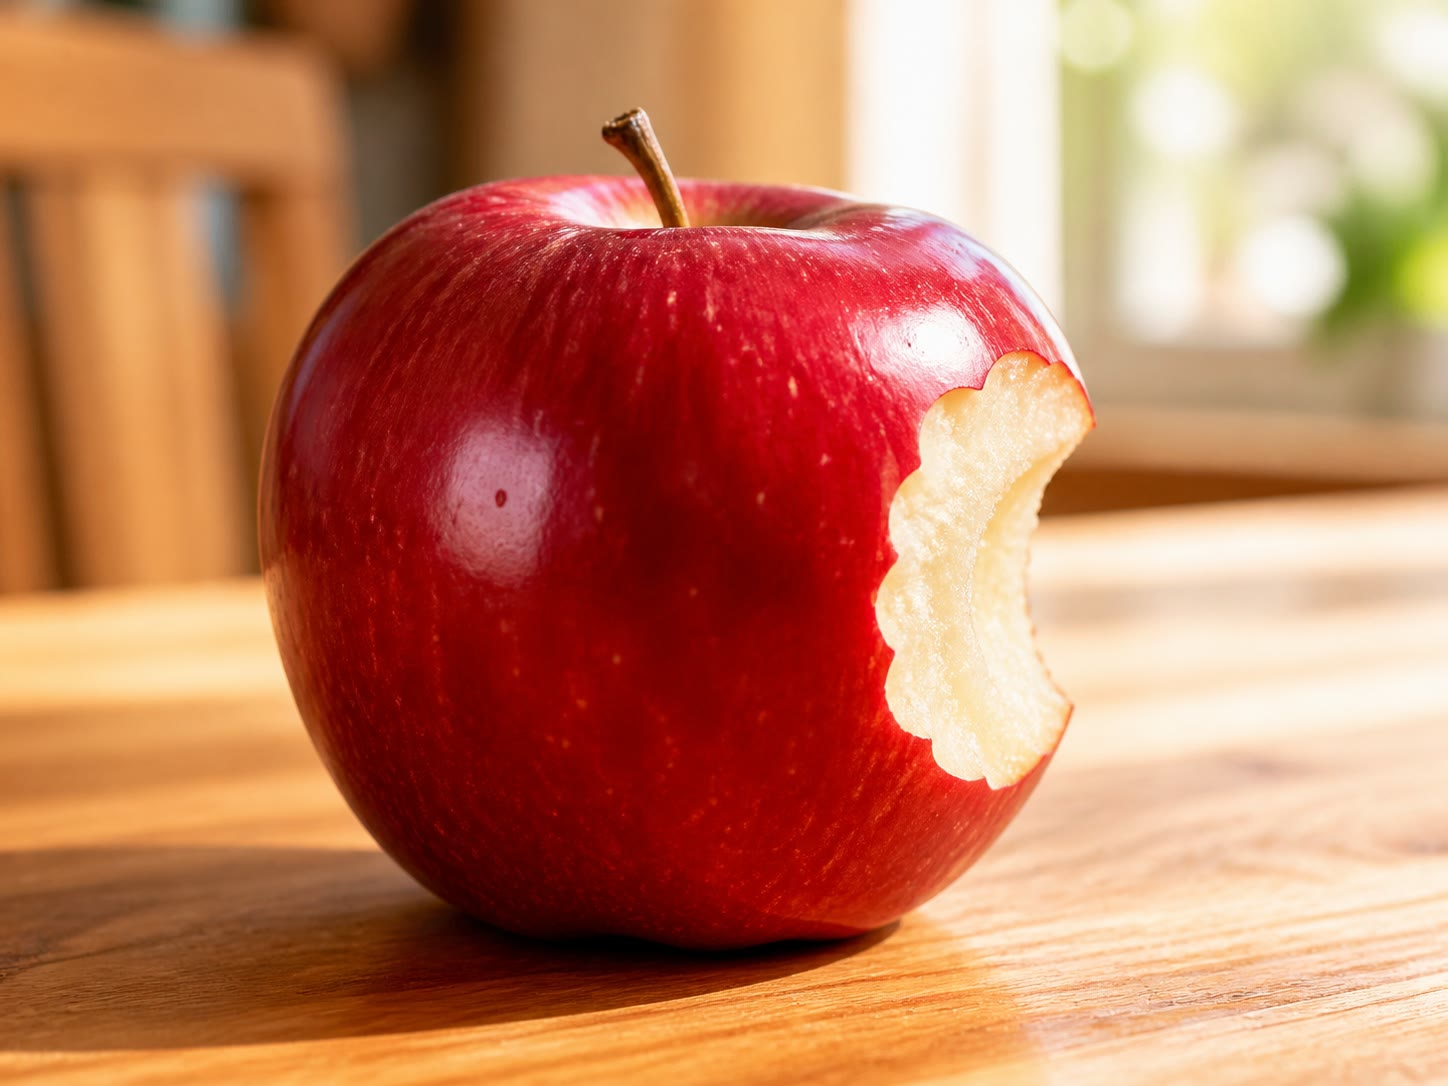
\includegraphics[width=0.52\linewidth]{images/book1/ai/g1-five-senses-apple.jpg}

{\small تفاحة واحدة للحواس الخمس جميعًا: العينان تريان حمرتها، واليد تحسّ بقشرتها الملساء، والأذنان سمعتا قضمتها الناقصة، والأنف تشمّ عطرها، واللسان يحتفظ بمذاقها.}
\end{omfigure}

\begin{example}[جرّب: نزهة الأصوات]\label{ex:g1:five-senses:sounds}
اجلس ساكنًا، وأغمض عينيك، وعدّ الأصوات من حولك مدّة قصيرة:
سيارة، وصوت إنسان، والريح، وأنفاسك أنت. حين تُغمض العينان تلتقط
الأذنان أصواتًا كانت العينان المشغولتان تُنسيك إياها. ويجد أكثر
الناس $4$ أو $5$ أصوات لم ينتبهوا إليها من قبل.
\end{example}

\begin{remark}[حواس تحمينا]\label{rem:g1:five-senses:danger}
الحواس حرّاس أيضًا. فالأنف تشمّ الدخان قبل أن ترى العين النار؛
والجلد يسحب اليد بعيدًا عن المقلاة الساخنة؛ والطعم المرّ ينذر
``لا تبتلع هذا''. ولا تذق شيئًا مجهولًا ولا تشمّه عن قصد أبدًا:
اسأل شخصًا كبيرًا أولًا. والحرّاس يعملون خير عمل حين نرفق بهم.
\end{remark}

\section{الملاحظة الدقيقة}

النظر ليس \omterm{def:g1:five-senses:observation}{ملاحظة} بعد. كلّنا \emph{رأى} دعسوقة؛ فمن يستطيع أن يقول
كم رِجلًا لها؟

\begin{definition}[الملاحظة]\label{def:g1:five-senses:observation}
أن \emph{تُلاحِظ}\index{ملاحظة} هو أن تستعمل حواسك بدقة وعن
قصد للإجابة عن سؤال --- ثم أن تقول أو ترسم ما انتبهت إليه بالضبط،
لا ما كنت تتوقعه. و\emph{الملاحظة}\index{ملاحظة} هي ما اكتشفه
النظر المتأنّي.
\end{definition}

\begin{method}[كيف تلاحظ]\label{met:g1:five-senses:how}
\begin{enumerate}
  \item اختر سؤالًا: \emph{كم رِجلًا للدعسوقة؟}
  \item انظر (أو أصغِ، أو المِس) على مهل، بلا عجلة؛
  \item قل ما تنتبه إليه بكلمات دقيقة: لا ``إنها صغيرة''،
        بل ``إنها أصغر من ظفري''؛
  \item ارسمه أو احكِه، لكي يتحقّق منه غيرك.
\end{enumerate}
\omterm{def:g1:five-senses:observation}{الملاحظة} الجيدة يستطيع صديقك أن يتحقّق منها: إذا نظرتما معًا
فلا بدّ أن تجدا $6$ أرجل.
\end{method}

\begin{example}[كلمات دقيقة]\label{ex:g1:five-senses:words}
قارن ``الحجر جميل'' بقولك ``الحجر رماديّ، أملس، مستدير، وأبرد من
يدي''. الجملة الثانية \omterm{def:g1:five-senses:observation}{ملاحظة}: يستطيع طفل آخر أن يلتقط ذلك الحجر
من بين سلّة كاملة.
\end{example}

\begin{omfigure}
\begin{tikzpicture}[scale=0.8]
  % six legs, three per side
  \draw[thick] (1.32,-0.45) -- ++(-30:0.45);
  \draw[thick] (0.9,-0.76) -- ++(-55:0.45);
  \draw[thick] (0.38,-0.92) -- ++(-75:0.45);
  \draw[thick] (-1.32,-0.45) -- ++(210:0.45);
  \draw[thick] (-0.9,-0.76) -- ++(235:0.45);
  \draw[thick] (-0.38,-0.92) -- ++(255:0.45);
  % body, wing split, spots
  \draw[thick, fill=omDef!12] (0,0) ellipse (1.5 and 0.95);
  \draw[thick, omDef] (0,0.95) -- (0,-0.95);
  \fill[omThm] (-0.55,0.3) circle (0.13);
  \fill[omThm] (-0.85,-0.25) circle (0.13);
  \fill[omThm] (0.5,0.4) circle (0.13);
  \fill[omThm] (0.75,-0.25) circle (0.13);
  % head and antennae
  \fill[omDef] (1.55,0) circle (0.3);
  \draw[thick] (1.75,0.18) .. controls (2.0,0.35) .. (2.1,0.55);
  \draw[thick] (1.78,-0.14) .. controls (2.05,-0.28) .. (2.18,-0.42);
  \node[right, font=\small] at (2.8,0.5)
    {كم نقطة؟ وكم رِجلًا؟};
  \node[right, font=\small] at (2.8,-0.5)
    {انظر على مهل، ثم عُدّ.};
\end{tikzpicture}

{\small \omterm{def:g1:five-senses:observation}{ملاحظة} دعسوقة: العين المتأنّية تعدّ $4$ نقاط على هذه
الواحدة --- و$6$ أرجل دائمًا.}
\end{omfigure}

\section{حين تُخدع الحواس}

الحواس رائعة، لكنها تُخدع. ولهذا بالضبط سنتعلّم في الفصول القادمة
أن \emph{نقيس}.

\begin{example}[مستقيمان]\label{ex:g1:five-senses:lines}
في الصورة أدناه، أيّ المستقيمين أطول؟ يجيب الجميع تقريبًا
``العلوي''. تحقّق الآن بخيط: المستقيمان متساويان في الطول تمامًا.
لقد خدعت رؤوسُ الأسهم العينَ.
\end{example}

\begin{omfigure}
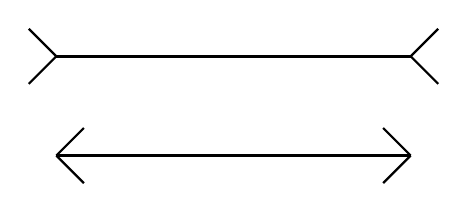
\begin{tikzpicture}[scale=0.9]
  \draw[very thick] (0,1.4) -- (5,1.4);
  \draw[thick] (0,1.4) -- ++(135:0.55) (0,1.4) -- ++(-135:0.55);
  \draw[thick] (5,1.4) -- ++(45:0.55) (5,1.4) -- ++(-45:0.55);
  \draw[very thick] (0,0) -- (5,0);
  \draw[thick] (0,0) -- ++(45:0.55) (0,0) -- ++(-45:0.55);
  \draw[thick] (5,0) -- ++(135:0.55) (5,0) -- ++(-135:0.55);
\end{tikzpicture}

{\small حيلة رؤوس الأسهم المشهورة: المستقيمان لهما الطول نفسه.
تحقّق بخيط!}
\end{omfigure}

\begin{example}[جرّب: ثلاث أوعية]\label{ex:g1:five-senses:bowls}
اطلب من شخص كبير أن يهيّئ ثلاثة أوعية ماء: واحد بارد، وواحد فاتر،
وواحد دافئ يُحتمل. ضع إحدى يديك في الوعاء البارد والأخرى في
الدافئ، وعُدّ على مهل حتى $20$. ثم ضع يديك معًا في الوعاء
الأوسط: الماء نفسه يبدو دافئًا ليد وباردًا للأخرى! لا يُوثق باللمس
وحده في الحارّ والبارد --- والفصل التالي يعالج هذه المسألة بعينها.
\end{example}

\begin{remark}[أعوان للحواس]\label{rem:g1:five-senses:tools}
يصنع الناس أدوات تساعد الحواس: النظّارة والعدسة المكبّرة تساعدان
العين، وسمّاعة الطبيب تساعد الأذن. وفي ما بعدُ من هذا الكتاب
ستفعل أدوات تُسمّى \emph{أجهزة} خيرًا من ذلك: ستحوّل النظر واللمس
إلى عدّ وقياس، والعدّ أصعب على الخداع بكثير.
\end{remark}

\section{تمارين}

\begin{exercise}[$\star$]\label{exo:g1:five-senses:1}
سمِّ الحواس الخمس، واذكر لكل واحدة عضو الجسم الذي يقوم بها.
\end{exercise}

\begin{exercise}[$\star$]\label{exo:g1:five-senses:2}
أيّ حاسة تخبرك: (أ) أن المذياع يعمل؟ (ب) أن الحساء شديد الملوحة؟
(ج) أن كنزتك خشنة؟ (د) أن الأضواء انطفأت؟
\end{exercise}

\begin{exercise}[$\star$]\label{exo:g1:five-senses:3}
كعكة تُخبز في الفرن، والباب مغلق، وأنت في غرفة أخرى. أيّ حاسة
تكتشفها أولًا؟ وأيّ الحواس تستعمل حين تنال قطعة منها أخيرًا؟
\end{exercise}

\begin{exercise}[$\star$]\label{exo:g1:five-senses:4}
قم بنزهة الأصوات في \cref{ex:g1:five-senses:sounds}: أغمض عينيك،
وعُدّ الأصوات حولك. كم صوتًا سمعت؟ وأيّها فاجأك؟
\end{exercise}

\begin{exercise}[$\star$]\label{exo:g1:five-senses:5}
أعطِ \omterm{def:g1:five-senses:observation}{ملاحظة} عن حذائك بثلاث كلمات دقيقة، كما في
\cref{ex:g1:five-senses:words}. و``جميل'' و``حلو'' ممنوعتان!
\end{exercise}

\begin{exercise}[$\star$]\label{exo:g1:five-senses:6}
تقول آنا: ``القطة ناعمة.'' ويقول بوب: ``القطة أحسن قطة.''
أيّ الجملتين \omterm{def:g1:five-senses:observation}{ملاحظة}، وأيّ حاسة صنعتها؟ وما الجملة الأخرى؟
\end{exercise}

\begin{exercise}[$\star$]\label{exo:g1:five-senses:7}
أيّ حاسة تنذرك بكل خطر من هذه: (أ) دخان في مكان ما من البيت؛
(ب) مقلاة أسخن من أن تُمسك؛ (ج) سيارة قادمة من خلفك؟
\end{exercise}

\begin{exercise}[$\star$]\label{exo:g1:five-senses:8}
يُغمض صديق عينيه. وتضع أمامه ملعقة وإسفنجة وحصاة، واحدة بعد
الأخرى. أيستطيع تسمية الثلاث باللمس وحده؟ وأيّها كان أسهلها
تعرّفًا؟
\end{exercise}

\begin{exercise}[$\star\star$]\label{exo:g1:five-senses:9}
انظر إلى المستقيمين في \cref{ex:g1:five-senses:lines}. اشرح
لصديقك كيف يتيقّن أيّ المستقيمين أطول من غير أن يثق بعينيه.
أتصلح طريقتك أيضًا لمقارنة مستقيم بخيط ملتوٍ؟
\end{exercise}
